
% Para elaborar este relatório, utilizei o template Sullivan Business Report, disponível em:
% https://www.latextemplates.com/template/sullivan-business-report
% Agradeço ao autor por disponibilizá-lo gratuitamente.

\documentclass[a4paper, 12pt]{CSSullivanBusinessReport}
\usepackage[portuguese]{babel}
\usepackage{longtable}
\usepackage{array} 
\usepackage{xcolor}
\definecolor{slightlyred}{RGB}{255,100,100}
\usepackage{hyperref}
\hypersetup{colorlinks=true, linkcolor=black, citecolor=black, urlcolor=black}

% Obs: as tabelas foram formatadas através da função xtable, do pacte de mesmo nome da linguagem de programação R. Para mais detalhes, consulte o código R.

%----------------------------------------------------------------------------------------
%   INFORMAÇÕES
%----------------------------------------------------------------------------------------

\reporttitle{Relatório de Análise} 
\reportsubtitle{Impactos da Proposta de Ajuste Salarial \\ da Carropel Implementos Rodoviários} 
\reportauthors{Relatório escrito e elaborado por\\\smallskip \href{https://gabrielmaia98.github.io/}{Gabriel Lima}}
\reportdate{25 de outubro de 2024} 

\rightheadercontent{\includegraphics[width=3cm]{logo.png}} 

%----------------------------------------------------------------------------------------

\begin{document}

%----------------------------------------------------------------------------------------
%	Capa
%----------------------------------------------------------------------------------------

\thispagestyle{empty} % Remove cabeçalhos e outros detalhes dessa página

\begin{fullwidth} 
	\vspace*{-0.075\textheight} 
	
	\hfill\includegraphics[width=5cm]{Images/logo.png} 

	\vspace{0.15\textheight}

	\parbox{0.9\fulltextwidth}{\fontsize{50pt}{52pt}\selectfont\raggedright\textbf{\reporttitle}\par} 
	
	\vspace{0.03\textheight} 
	
	{\LARGE\textit{\textbf{\reportsubtitle}}\par} 
	
	\vfill 
	
	{\Large\reportauthors\par} 
	
	\vfill\vfill\vfill 
	
	{\large\reportdate\par} 
\end{fullwidth}

\newpage

%----------------------------------------------------------------------------------------
%	Aviso e Nota de Copyright
%----------------------------------------------------------------------------------------

\thispagestyle{empty} 

\begin{twothirdswidth} 
	\footnotesize 
	
	\subsection*{Aviso de Sigilo e Uso Restrito}

Este relatório contém informações confidenciais relacionadas à folha de pagamento da Carropel Implementos Rodoviários. O acesso a este documento é restrito a pessoas autorizadas pela empresa, e qualquer divulgação ou uso não autorizado das informações aqui contidas é estritamente proibido. Os destinatários deste relatório devem garantir a proteção dos dados e utilizá-los exclusivamente para os fins previstos pela Carropel.

    \subsubsection*{Nota Adicional}

Esta versão do relatório foi criada para fins de portfólio e contém dados anonimizados. No entanto, o uso do documento permanece restrito e sujeito às mesmas condições de sigilo e proteção de informações, conforme mencionado anteriormente. Isto incluí restrições sobre distribuição e utilização.


	\subsection*{Copyright}
	
	\textcopyright~[2024] [Carropel Implementos Rodoviários] 
	
Este documento é protegido por direitos autorais e a propriedade intelectual dos conteúdos aqui apresentados pertence à Carropel Implementos Rodoviários. É proibida a reprodução total ou parcial deste relatório sem a autorização expressa da empresa. A utilização de qualquer parte deste documento para fins não autorizados poderá resultar em ações legais, conforme a legislação vigente.

	
	\subsection*{Contato}
	
	Av. Anel Viário, nº 360\\
	Toco, Caucaia/CE\\
	CEP: 61663-135

	Telefone Comercial: +55 (85) 3497-3200 
	
	Email: carropel@carropel.com.br
	
	\vfill 
	
	\subsubsection*{Changelog}
	
	\scriptsize 
	
	\begin{tabular}{@{} L{0.05\linewidth} L{0.12\linewidth} L{0.6\linewidth} @{}} 
		\toprule
		v1.0 & 25-10-2024 & Entrega inicial \\
            v1.1 & 25-10-2024 & Versão anonimizada \\
		\bottomrule
	\end{tabular}
\end{twothirdswidth}

\newpage

%----------------------------------------------------------------------------------------
%	Conteúdo - Sumário
%----------------------------------------------------------------------------------------

\begin{twothirdswidth} 
	\tableofcontents 
\end{twothirdswidth}

\newpage

%----------------------------------------------------------------------------------------
%	Seção 1
%----------------------------------------------------------------------------------------

\section{Introdução} 
\begin{fullwidth}
Apresentarei aqui os resultados obtidos ao analisar a proposta de reajuste salarial da Carropel Implementos Rodoviários para o último trimestre de 2024. A proposta tem como base a padronização dos salários no setor de produção. Utilizei as planilhas fornecidas por Fernando Levy, que tiveram por origem o setor administrativo da empresa. Formatei-as utilizando a linguagem de programação R, fiz os gráficos aqui apresentados com o ggplot2 e o bbplot, e por último elaborei este relatório utilizando \LaTeX.

%----------------------------------------------------------------------------------------
%	Seção 2 
%----------------------------------------------------------------------------------------

\section{Reajuste por categoria} 


\subsection{Valores investidos}

Aqui apresento gráficos que ilustrarão as mudanças. Comecemos pelo montante total a ser investido\sidenote[\hspace{0cm}][1.5cm]{Como podemos observar, haverá um aumento no valor total gasto. Hoje, a folha de pagamento do setor de produção resulta em um total de R\$ 93.542,00 mensais. Caso venha a ser efetivada a mudança, o novo total mensal será de R\$ 106.600,00, ou seja, haverá um aumento de aproximadamente 15\% da folha salarial, ou um crescimento de R\$ 174.255,00 para as despesas anuais. \\\smallskip Resumindo: \\\medskip \begin{itemize}[leftmargin=*]\item Aumento de 15\%. \item R\$ 14.521,25 por mês. \item R\$ 106.600,00 por ano.\end{itemize}}:

%----------------------------------------------------------------------------------------
%	Figura 1
%----------------------------------------------------------------------------------------


\begin{figure}[H] % [H] força figura ficar onde foi colocada
	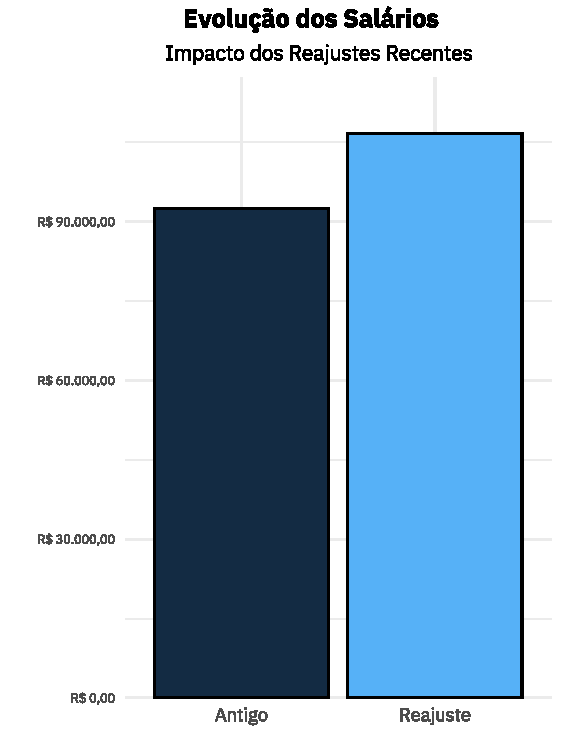
\includegraphics[width=\linewidth, height=0.5\textheight, keepaspectratio]{Images/Rplot.pdf}
	\caption{Evolução do gasto mensal em folha de pagamento do setor de produção.}
	\label{fig:reajustetotalmes} 
 \end{figure}

\newpage


\subsection{Efeitos nas categorias} 
Agora observemos como o reajuste afetará cada categoria separadamente. Por categoria, entenda Função e Nível. Comecemos com uma tabela exibindo cada categoria, a quantidade total de funcionários nelas presentes, o total mensal que será investido em cada uma para realizar a mudança, o novo valor proposto para cada nível, e a antiga média salarial. 

%----------------------------------------------------------------------------------------
%	Tabela 1
%----------------------------------------------------------------------------------------

\begin{table}[H] 
	\caption{Reajuste Salarial por Categoria}
	\begin{tabular}{L{0.25\linewidth} R{0.1\linewidth} R{0.23\linewidth} R{0.2\linewidth} R{0.3\linewidth}} 
		\toprule
		\textbf{Categoria} & \textbf{QTD} & \textbf{Total} & \textbf{Proposta} & \textbf{Média Antiga}\\
		\midrule
  Auxiliar 1 &   5 & R\$ 0.00 & R\$ 1450.00 & R\$ 1450.00 \\ 
  Auxiliar 2 &   3 & R\$ 450.00 & R\$ 1600.00 & R\$ 1450.00 \\ 
  Auxiliar 3 &   4 & R\$ 487.51 & R\$ 1750.00 & R\$ 1628.12 \\ 
  Eletricista 1 &   1 & R\$ 150.00 & R\$ 1600.00 & R\$ 1450.00 \\ 
  Eletricista 2 &   1 & R\$ 400.00 & R\$ 1850.00 & R\$ 1450.00 \\ 
  Encarregado &   6 & R\$ 4723.24 & R\$ 2800.00 & R\$ 2012.79 \\ 
  Montador 1 &   8 & R\$ 1570.51 & R\$ 1850.00 & R\$ 1653.68 \\ 
  Montador 2 &   7 & R\$ 2837.21 & R\$ 2200.00 & R\$ 1794.68 \\ 
  Montador 3 &   5 & R\$ 1749.25 & R\$ 2500.00 & R\$ 2150.15 \\ 
  Operador 1 &   1 & R\$ 0.00 & R\$ 1900.00 & R\$ 1900.00 \\ 
  Operador 3 &   2 & R\$ 1068.77 & R\$ 2500.00 & R\$ 1965.61 \\ 
  Pintor 1 &   1 & R\$ 0.00 & R\$ 1450.00 & R\$ 1450.00 \\ 
  Pintor 2 &   2 & R\$ 245.08 & R\$ 1700.00 & R\$ 1577.46 \\ 
  Pintor 3 &   1 & R\$ 231.03 & R\$ 1850.00 & R\$ 1618.97 \\ 
  Soldador 1 &   3 & \textcolor{slightlyred}{R\$ -464.52} & R\$ 2000.00 & R\$ 2154.84 \\ 
  Soldador 2 &   1 & R\$ 100.00 & R\$ 2400.00 & R\$ 2300.00 \\ 
  Soldador 3 &   1 & R\$ 508.65 & R\$ 2600.00 & R\$ 2091.35 \\ 
  \midrule
 \textbf{Total} & 52 & R\$ 14.521,25 & & \\
		\bottomrule
	\end{tabular}
	\label{tab:categorias}
\end{table}
\end{fullwidth}

Como podemos observar, os maiores investimentos\sidenote[\hspace{0cm}][0cm]{Maiores investimentos por categoria: \\\medskip \begin{itemize}[leftmargin=*]\item Encarregados: receberão R\$ 4.723,24 a mais por mês. \item Montadores de nível 2 receberão R\$ 2.837,21 a mais. \item Montadores de nível 3: R\$ 1.749,25. \%.\end{itemize}} serão realizados com os funcionários nos cargos de encarregados, montadores de nível 2, 3 e 1 e operadores de nível 3, respectivamente. O valor total investido, com base na soma dos reajustes, seria de R\$ 14.056,73 mensais e beneficiaria, ao todo, 52 funcionários. Observe, porém a presença de valores negativos, que ocorrem devido a funcionários com salário acumulado acima da categoria. Desconsiderando uma redução salarial, o verdadeiro valor investido será R\$  R\$ 14.521,25.

\begin{fullwidth}

\paragraph{Visualizando as mudanças.} Podemos observar os maiores investimentos e suas proporções, comparados aos outros, a partir do seguinte gráfico:

%----------------------------------------------------------------------------------------
%	Figura 2
%----------------------------------------------------------------------------------------

\vspace{-0.3cm}
\begin{figure*}[H] 
	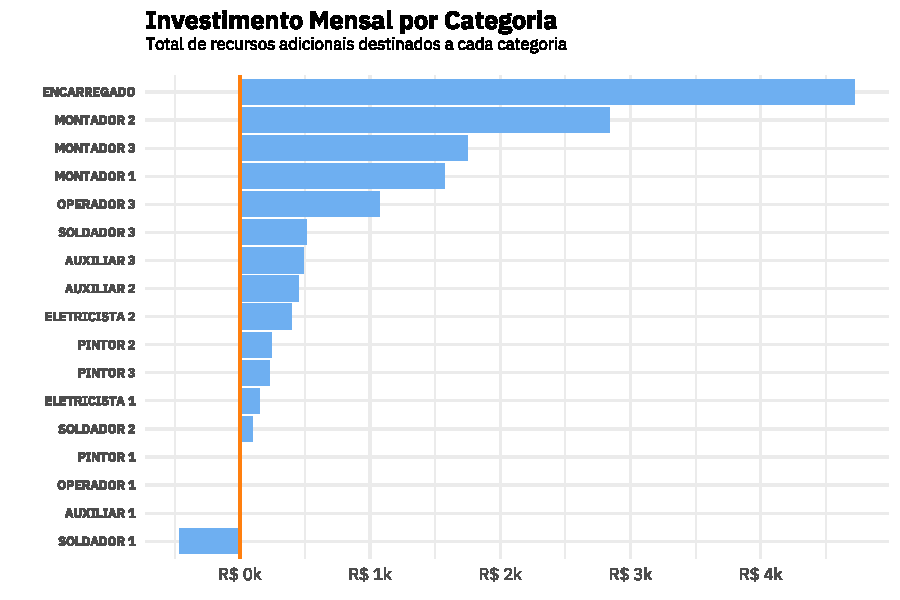
\includegraphics[width=\linewidth, height=\textheight, keepaspectratio]{Images/Rplot01.pdf}
	\caption{Reajuste por categoria}
	\label{fig:reajustecategoria} 
 \end{figure*}

\vspace{-0.7cm} % melhor espaçamento

Ressalto que o gráfico acima representa o aumento no valor recebido por cada categoria, e não o valor mensal total a ser recebido. Trata-se da diferença entre (1) o que a categoria recebe e (2) o que receberá com o reajuste, e quanto a empresa precisará investir a mais em cada uma. A categoria de soldador 1 provavelmente é a que possui mais funcionários com excepcionais. O gráfico não considera a decisão de mantê-los, por isso o valor negativo. Agora, vejamos com mais atenção como cada categoria influenciou o valor final:

%----------------------------------------------------------------------------------------
%	Tabela 2
%----------------------------------------------------------------------------------------


\begin{table}[h]
    \centering
    \caption{Soma dos valores pagos antes e após o reajuste.}
        \begin{tabular}{|c|c|c|c|}
        \hline
        \textbf{Função} & \textbf{Nível 1} & \textbf{Nível 2} & \textbf{Nível 3} \\ \hline
        Auxiliar & 7.250 → 7.250 & 4.350 → 4.800 & 6.512 → 7.000 \\ \hline
        Eletricista & 1.450 → 1.600 & 1.450 → 1.850 & \\ \hline
        Encarregado & 12.077 → 16.800 & & \\ \hline
        Montador & 13.229 → 14.800 & 12.563 → 15.400 & 10.751 → 12.500 \\ \hline
        Operador & 1.900 → 1.900 & 3.931 → 5.000 & \\ \hline
        Pintor & 1.450 → 1.450 & 3.155 → 3.400 & 1.619 → 1.850 \\ \hline
        Soldador & 6.465 → 6.000 & 2.300 → 2.400 & 2.091 → 2.600 \\ \hline
    \end{tabular}
	\label{tab:reajuste}
\end{table}

\newpage

\paragraph{Custos Totais.} O custo de cada categoria para o total da folha de pagamento pode ser visualizado do seguinte modo:

%----------------------------------------------------------------------------------------
%	Figura 3
%----------------------------------------------------------------------------------------

\begin{figure*}[H]
	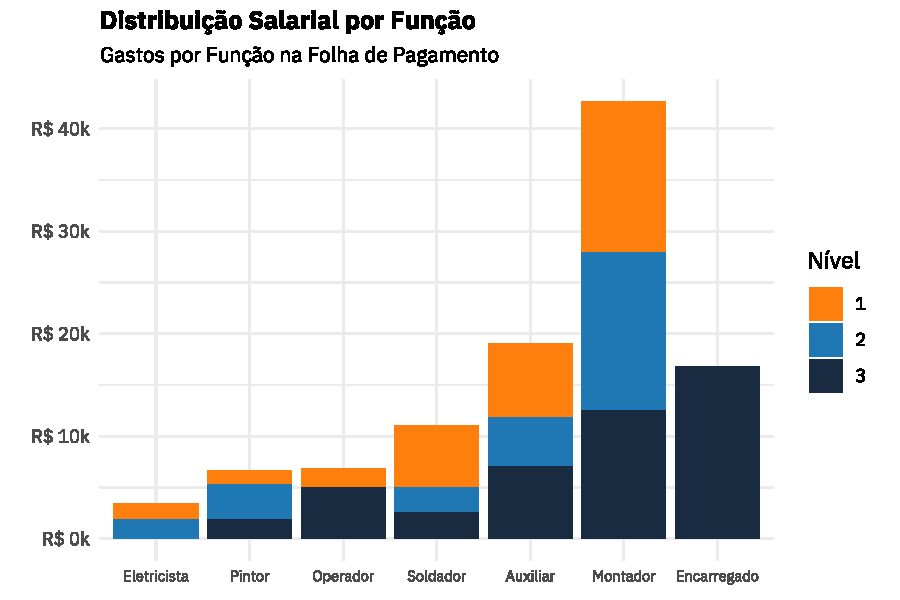
\includegraphics[width=\linewidth, height=\textheight, keepaspectratio]{Images/dist.pdf}
	\caption{Desdobramento da Folha Salarial por Função}
	\label{fig:salariopfuncao} % Label for referencing this figure in the text automatically
 \end{figure*}

%----------------------------------------------------------------------------------------
%	Tabela 4
%----------------------------------------------------------------------------------------

\vspace{-0.7cm}
A seguir, apresento uma tabela com os dados numéricos, a fim de facilitar a consulta.

\begin{table}[h]
    \centering
    \caption{Distribuição Salarial por Categoria}
    \begin{minipage}{0.5\textwidth}
        \centering
        \begin{tabular}{lr}
            \toprule
            \textbf{Categoria} & \textbf{Total} \\ 
            \midrule
            Auxiliar 1 & R\$ 7.250,00 \\ 
            Auxiliar 2 & R\$ 4.800,00 \\ 
            Auxiliar 3 & R\$ 7.000,00 \\ 
            Eletricista 1 & R\$ 1.600,00 \\ 
            Eletricista 2 & R\$ 1.850,00 \\ 
            Encarregado & R\$ 16.800,00 \\ 
            Montador 1 & R\$ 14.800,00 \\ 
            Montador 2 & R\$ 15.400,00 \\ 
            Montador 3 & R\$ 12.500,00 \\ 
           \bottomrule
        \end{tabular}
    \end{minipage}\hfill
    \begin{minipage}{0.5\textwidth}
        \centering
        \begin{tabular}{lr}
            \toprule
            \textbf{Categoria} & \textbf{Total} \\ 
            \midrule
            Operador 1 & R\$ 1.900,00 \\ 
            Operador 2 & R\$ - - - - - - - \\
            Operador 3 & R\$ 5.000,00 \\ 
            Pintor 1 & R\$ 1.450,00 \\ 
            Pintor 2 & R\$ 3.400,00 \\ 
            Pintor 3 & R\$ 1.850,00 \\ 
            Soldador 1 & R\$ 6.000,00 \\ 
            Soldador 2 & R\$ 2.400,00 \\ 
            Soldador 3 & R\$ 2.600,00 \\
            \bottomrule
        \end{tabular}
        \label{tab:distrib}
    \end{minipage}
\end{table}\sidenote[ ][-8cm]{Observamos que a maior parte dos recursos financeiros da folha salarial se concentra entre os montadores, que acumulam acima de R\$ 40.000,00. Os encarregados, porém, são os mais bem pagos, considerando que estão em menor número para o total acumulado do salário. Os gastos com eletricistas são poucos.}

\subsection{Análise por setor}

Também podemos analisar a distribuição de verbas por setores e os que serão mais beneficiados com o reajuste, utilizando o mesmo estilo de tabelas e visualizações.

%----------------------------------------------------------------------------------------
%	Tabela 4
%----------------------------------------------------------------------------------------

\begin{table}[h]
\centering
\caption{Impacto por setor}
\begin{tabular}{lrrrr}
    \toprule
\textbf{Setor} & \textbf{QTD} & \textbf{Valor Anterior} & \textbf{Reajuste} & \textbf{Novo Valor} \\ 
    \midrule
  Baús & 12 & R\$ 21.002,74 & R\$ 2.197,26 & R\$ 23.200,00 \\ 
  Elétrica & 2 & R\$ 2.900,00 & R\$ 550,00 & R\$ 3.450,00 \\ 
  Encarroçamento & 1 & R\$ 1.450,00 & R\$ 400,00 & R\$ 1.850,00 \\ 
  Entre-Eixo & 2 & R\$ 3.415,61 & R\$ 1.584,39 & R\$ 5.000,00 \\ 
  Hidráulicos & 2 & R\$ 4.521,78 & R\$ 178,22 & R\$ 4.700,00 \\ 
  Metalúrgica & 15 & R\$ 27.197,68 & R\$ 4.552,32 & R\$ 3.1750,00 \\ 
  Pesados & 9 & R\$ 18.038,47 & R\$ 1.811,53 & R\$ 19.850,00 \\ 
  Pintura & 5 & R\$ 8.025,26 & R\$ 1.474,74 & R\$ 9.500,00 \\ 
  Reforma & 4 & R\$ 5.991,73 & R\$ 1.308,27 & R\$ 7.300,00 \\ 
   \hline
\end{tabular}
\label{tab:setor}
\end{table}


A visualização disposta abaixo\sidenote[1][4cm]{O mapa de radar não mostra os valores com exatidão, mas eles estão disponíveis na tabela acima. O uso principal dessa visualização é comparativo, ela demonstra bem a diferença entre cada setor, tomando um deles como parâmetro do maior valor possível.} representa o quanto o total das verbas está distribuído para cada setor. Tome como referência o valor máximo na extremidade e o valor mínimo no centro. Resumindo, os setores de metalurgia, pesados e baús recebem a maior parte do orçamento da empresa. Também são os setores com mais funcionários. Tudo normal por aqui.

%----------------------------------------------------------------------------------------
%	Figura 4
%----------------------------------------------------------------------------------------


\vspace{-0.5cm}
\begin{figure*}[H] 
	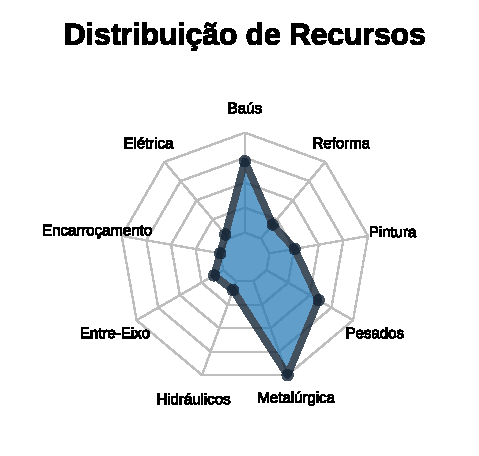
\includegraphics[width=0.6\linewidth, height=\textheight, keepaspectratio]{Images/Gastos-2.pdf}
	\caption{Radar dos Gastos}
	\label{fig:gastos} 
 \end{figure*}

\vspace{-0.7cm}
Aqui veremos o quanto cada função e nível recebem da verba salarial e como isso será modificado. No geral, as alterações parecem proporcionais entre os setores, com o da metalurgia sendo um pouco mais beneficiado que os outros em termos percentuais, e consideravelmente mais, em números absolutos. 

%----------------------------------------------------------------------------------------
%	Figura 5
%----------------------------------------------------------------------------------------

\begin{figure*}[H] 
	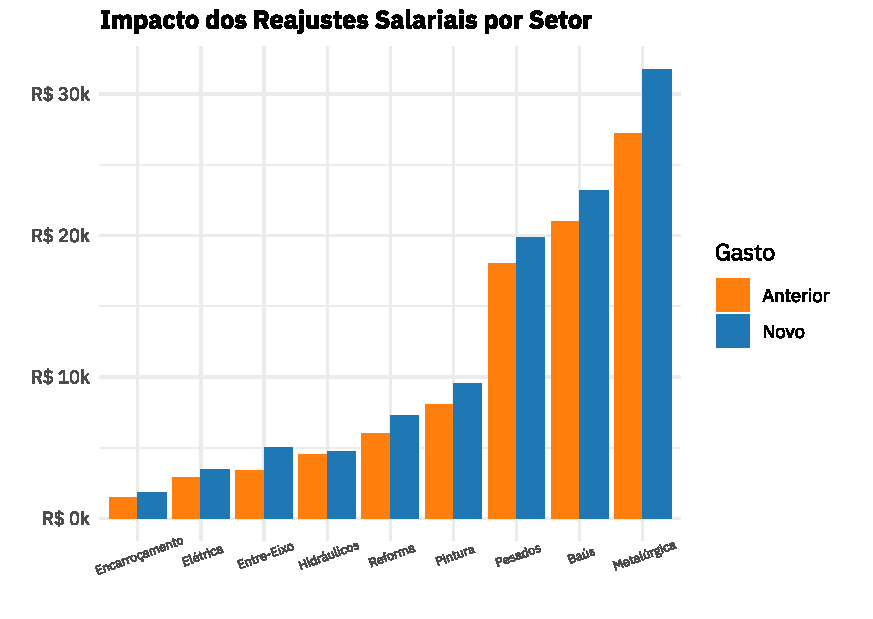
\includegraphics[width=\linewidth, height=\textheight, keepaspectratio]{Images/compar.pdf}
	\caption{Comparativo do total gasto em cada setor}
	\label{fig:comparsetor} 
 \end{figure*}
\vspace{-0.7cm}

\subsection{Conclusão}
\vspace{-0.4cm}
Caso venha a termo conforme o que foi proposto, o reajuste impactará a empresa do seguinte modo:

\begin{itemize}
	\item Um aumento de R\$ 14.521,25 por mês;
            \begin{itemize}
            \item Um crescimento de 15\% em relação ao modelo atual;
            \item Resultando em R\$ 106.600,00 a mais por ano.
            \end{itemize}
	\item Os encarregados serão a categoria mais beneficiada;
            \begin{itemize}
            \item Passarão a receber R\$ 4.723,24 a mais todo mês;
            \item E serão seguidos pelos montadores.
            \end{itemize}
	\item Nenhum setor ultrapassará outro em remuneração, exceto o de entre-eixos;
            \begin{itemize}
            \item Metalurgia, baús e pesados continuarão com mais verbas;
            \item e o setor de entre-eixos ultrapassará o de hidráulicos.
            \end{itemize}

\end{itemize}


%% ---------------------------------------------------------------------------------------------------

\newpage

%----------------------------------------------------------------------------------------
%	Seção 3
%----------------------------------------------------------------------------------------

\section{Funcionários beneficiados}

\paragraph{Introdução.}Aqui consideraremos as alterações e os impactos que elas poderão causar para os funcionários e suas carreiras. Começaremos analisando o reajuste para cada categoria com um gráfico de hálter, em seguida, gráficos de barras comparativos que demonstrarão as possibilidades de carreira e remuneração, e por último uma tabela listando os funcionários beneficiados.

\subsection{Uma análise gráfica das perspectivas de carreira na Carropel}

Do ponto de vista dos funcionários beneficiados, podemos entender os aumentos do seguinte modo:

%----------------------------------------------------------------------------------------
%	Figura 6
%----------------------------------------------------------------------------------------

\begin{figure*}[H] 
	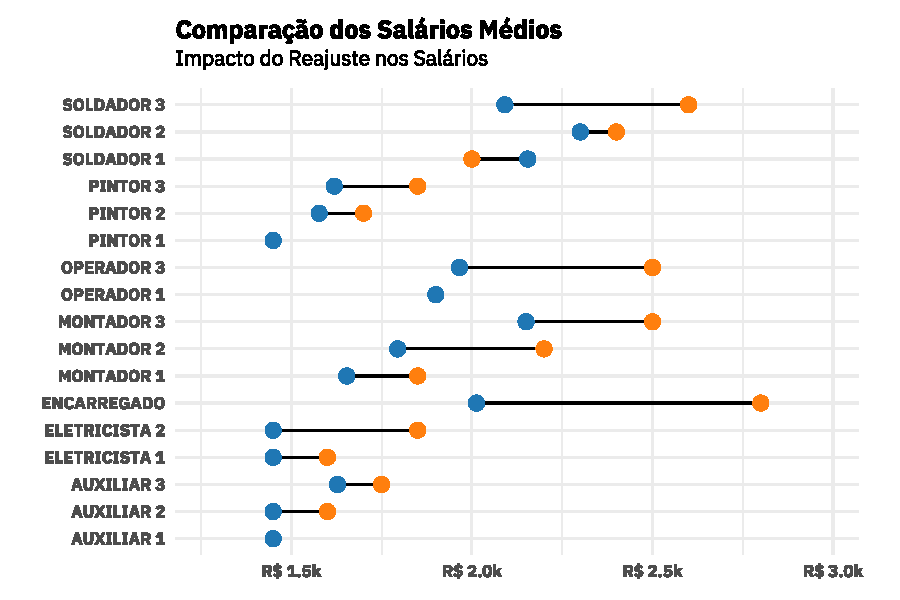
\includegraphics[width=\linewidth, height=\textheight, keepaspectratio]{Images/Rplot02.pdf}
	\caption{Comparativo das Médias de Salário Atual e Proposto}
	\label{fig:compasal} 
 \end{figure*}


\vspace{-0.7cm}
O ponto azul representa o salário atual, e o ponto laranja o salário após o reajuste. Note que esse é o impacto da perspectiva deles mais do que da empresa. Os encarregados serão os que terão o maior reajuste, seguidos pelos operadores e soldadores do nível 3. Este é um gráfico que ilustra a tabela \ref{tab:categorias}, mas de outra perspectiva. 

\paragraph{Perspectivas de Progressão} É essencial para a empresa que bons funcionários tenham espaço para evolução e sejam recompensados pelos seus esforços. Caso o reajuste seja implementado, as carreiras serão afetadas do modo explicitado na página a seguir. Note que todos os gráficos possuem a mesma legenda e o mesmo eixo vertical.

%----------------------------------------------------------------------------------------
%	Figura 7 - página inteira
%----------------------------------------------------------------------------------------

\begin{figure*}[H] 
	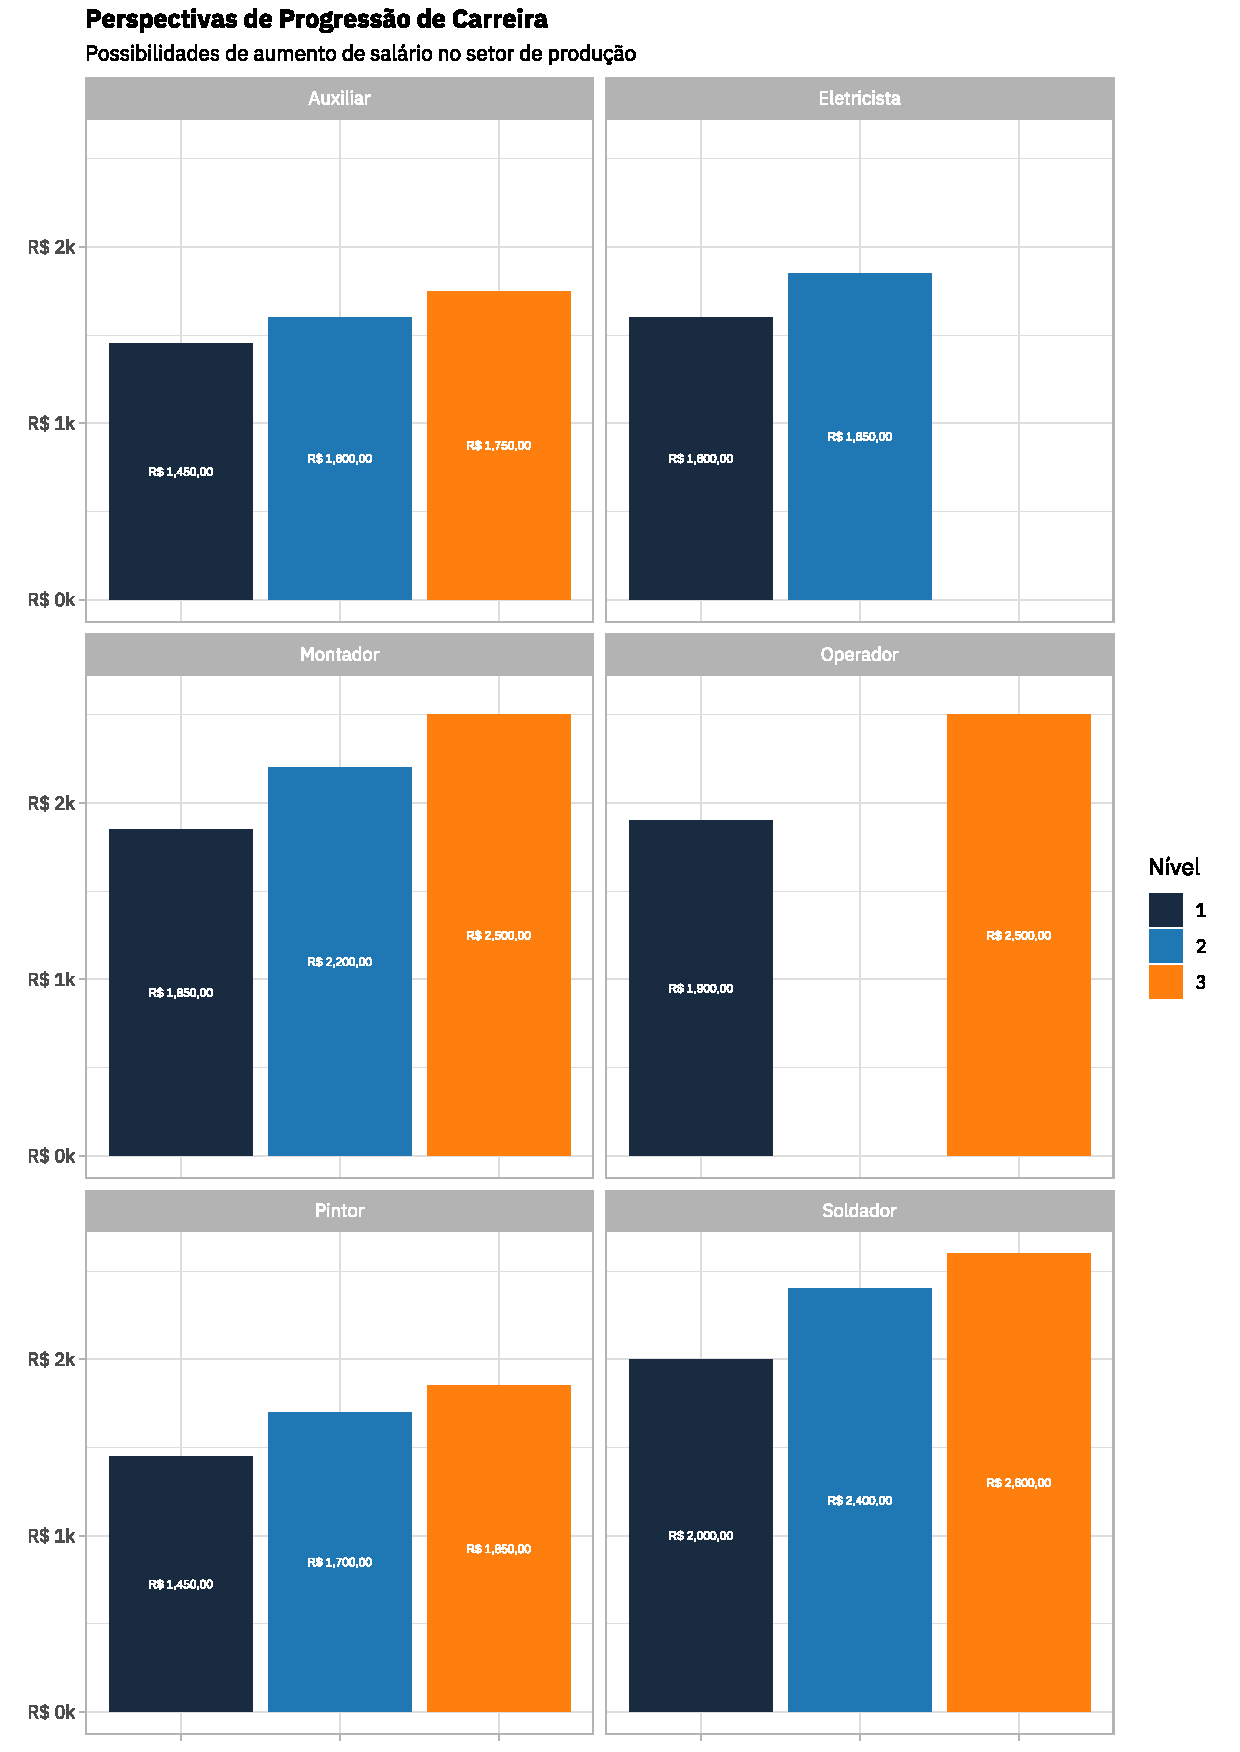
\includegraphics[width=\linewidth, height=\textheight, keepaspectratio]{Images/Progcarr.pdf}
	\caption{Progrssão de Carreira na Carropel}
	\label{fig:progcarr} 
 \end{figure*}
\vspace{-0.7cm}

\subsection{Tabela dos ajustes para cada funcionário}

Por fim, para fins de consulta, disponibilizarei a tabela dos funcionários, seus respectivos salários antetiores e posteriores e o valor do reajuste.

%----------------------------------------------------------------------------------------
%	Tabela 5
%----------------------------------------------------------------------------------------


\begin{longtable}{|L{0.3\linewidth}|R{0.2\linewidth}|R{0.2\linewidth}|R{0.2\linewidth}|}
\caption{Tabela dos ajustes por funcionário}
\hline
\textbf{Nome} & \textbf{Salário Atual} & \textbf{Proposta} & \textbf{Reajuste}\\
\hline
\endhead
  Funcionário 1 & R\$ 1.864,52 & R\$ 2.800,00 & R\$  935,48 \\ 
  Funcionário 2 & R\$ 1.800,00 & R\$ 2.200,00 & R\$  400,00 \\ 
  Funcionário 3 & R\$ 2.211,23 & R\$ 2.500,00 & R\$  288,77 \\ 
  Funcionário 4 & R\$ 2.016,68 & R\$ 2.500,00 & R\$  483,32 \\ 
  Funcionário 5 & R\$ 1.450,00 & R\$ 1.600,00 & R\$  150,00 \\ 
  Funcionário 6 & R\$ 1.762,49 & R\$ 1.750,00 & \textcolor{slightlyred}{R\$  -12,49} \\ 
  Funcionário 7 & R\$ 2.287,24 & R\$ 2.800,00 & R\$  512,76 \\ 
  Funcionário 8 & R\$ 2.100,00 & R\$ 1.850,00 & \textcolor{slightlyred}{R\$ -250,00} \\ 
  Funcionário 9 & R\$ 2.091,35 & R\$ 2.600,00 & R\$  508,65 \\ 
  Funcionário 10 & R\$ 1.712,00 & R\$ 2.800,00 & R\$ 1.088,00 \\ 
  Funcionário 11 & R\$ 1.450,00 & R\$ 1.450,00 & R\$    0,00 \\ 
  Funcionário 12 & R\$ 1.620,00 & R\$ 1.850,00 & R\$  230,00 \\ 
  Funcionário 13 & R\$ 1.641,73 & R\$ 2.200,00 & R\$  558,27 \\ 
  Funcionário 14 & R\$ 1.654,92 & R\$ 1.700,00 & R\$   45,08 \\ 
  Funcionário 15 & R\$ 1.800,00 & R\$ 1.750,00 & \textcolor{slightlyred}{R\$ -50,00} \\ 
  Funcionário 16 & R\$ 2.070,56 & R\$ 2.500,00 & R\$  429,44 \\ 
  Funcionário 17 & R\$ 1.593,87 & R\$ 1.850,00 & R\$  256,13 \\ 
  Funcionário 18 & R\$ 2.300,00 & R\$ 2.400,00 & R\$  100,00 \\ 
  Funcionário 19 & R\$ 1.450,00 & R\$ 1.450,00 & R\$    0,00 \\ 
  Funcionário 20 & R\$ 1.500,00 & R\$ 1.700,00 & R\$  200,00 \\ 
  Funcionário 21 & R\$ 1.720,00 & R\$ 2.500,00 & R\$  780,00 \\ 
  Funcionário 22 & R\$ 2.389,88 & R\$ 2.800,00 & R\$  410,12 \\ 
  Funcionário 23 & R\$ 2.021,75 & R\$ 2.800,00 & R\$  778,25 \\ 
  Funcionário 24 & R\$ 1.450,00 & R\$ 1.600,00 & R\$  150,00 \\ 
  Funcionário 25 & R\$ 1.450,00 & R\$ 1.850,00 & R\$  400,00 \\ 
  Funcionário 26 & R\$ 1.450,00 & R\$ 2.200,00 & R\$  750,00 \\ 
  Funcionário 27 & R\$ 1.801,37 & R\$ 2.800,00 & R\$  998,63 \\ 
  Funcionário 28 & R\$ 1.450,00 & R\$ 1.450,00 & R\$    0,00 \\ 
  Funcionário 29 & R\$ 1.450,00 & R\$ 1.850,00 & R\$  400,00 \\ 
  Funcionário 30 & R\$ 1.865,58 & R\$ 2.200,00 & R\$  334,42 \\ 
  Funcionário 31 & R\$ 1.618,97 & R\$ 1.850,00 & R\$  231,03 \\ 
  Funcionário 32 & R\$ 2.300,00 & R\$ 2.500,00 & R\$  200,00 \\ 
  Funcionário 33 & R\$ 2.721,78 & R\$ 2.500,00 & \textcolor{slightlyred}{R\$ -221,78} \\ 
  Funcionário 34 & R\$ 1.641,73 & R\$ 2.500,00 & R\$  858,27 \\ 
  Funcionário 35 & R\$ 1.450,00 & R\$ 1.450,00 & R\$    0,00 \\ 
  Funcionário 36 & R\$ 1.593,87 & R\$ 1.850,00 & R\$  256,13 \\ 
  Funcionário 37 & R\$ 1.450,00 & R\$ 1.750,00 & R\$  300,00 \\ 
  Funcionário 38 & R\$ 2.300,00 & R\$ 2.000,00 & \textcolor{slightlyred}{R\$ -300,00} \\ 
  Funcionário 39 & R\$ 1.700,00 & R\$ 1.850,00 & R\$  150,00 \\ 
  Funcionário 40 & R\$ 1.721,75 & R\$ 1.850,00 & R\$  128,25 \\ 
  Funcionário 41 & R\$ 1.450,00 & R\$ 1.600,00 & R\$  150,00 \\ 
  Funcionário 42 & R\$ 1.864,52 & R\$ 2.000,00 & R\$  135,48 \\ 
  Funcionário 43 & R\$ 2.300,00 & R\$ 2.000,00 & \textcolor{slightlyred}{R\$ -300,00} \\ 
  Funcionário 44 & R\$ 1.450,00 & R\$ 1.600,00 & R\$  150,00 \\ 
  Funcionário 45 & R\$ 2.027,67 & R\$ 2.200,00 & R\$  172,33 \\ 
  Funcionário 46 & R\$ 1.900,00 & R\$ 1.900,00 & R\$    0,00 \\ 
  Funcionário 47 & R\$ 1.450,00 & R\$ 1.450,00 & R\$    0,00 \\ 
  Funcionário 48 & R\$ 1.500,00 & R\$ 1.750,00 & R\$  250,00 \\ 
  Funcionário 49 & R\$ 1.703,61 & R\$ 2.200,00 & R\$  496,39 \\ 
  Funcionário 50 & R\$ 2.074,20 & R\$ 2.200,00 & R\$  125,80 \\ 
  Funcionário 51 & R\$ 1.450,00 & R\$ 1.450,00 & R\$    0,00 \\ 
  Funcionário 52 & R\$ 1.450,00 & R\$ 1.850,00 & R\$  400,00 \\ 
\hline
\textbf{Total} & R\$ 92.543,27 & R\$ 106.600,00 & R\$ 14.056,73 \\
\hline
\end{longtable}	

\subsection{Conclusão}

Conseguimos analisar em mais detalhes a proposta salarial e como ela afetaria setores, categorias, e funcionários. A partir disso, espera-se que a administração da empresa possa realizar uma decisão justa e bem informada quanto à folha salarial de seu setor de produção, considerando fatores que fogem ao escopo dessa análise numérica e gráfica. Agradeço ao Sr. Fernando Levy pela oportunidade de contribuir com a empresa e a todo o setor administrativo e gestores da Carropel.

\end{fullwidth}

\end{document}
